\subsection{Example of Importance Sampling}

\begin{frame}{Example of Importance Sampling -- Estimate Distribution}

Estimate the Beta Function -- $beta(2, 11)$, and suppose we do not know the equation. \\
We have two proposal options:\\
(1) Uniform Distribution;\\
(2) $beta(2,11)$ distribution itself.

\end{frame}

\begin{frame}{Example of Importance Sampling -- Estimate Distribution}
\begin{figure}[ht]
		  \centering
          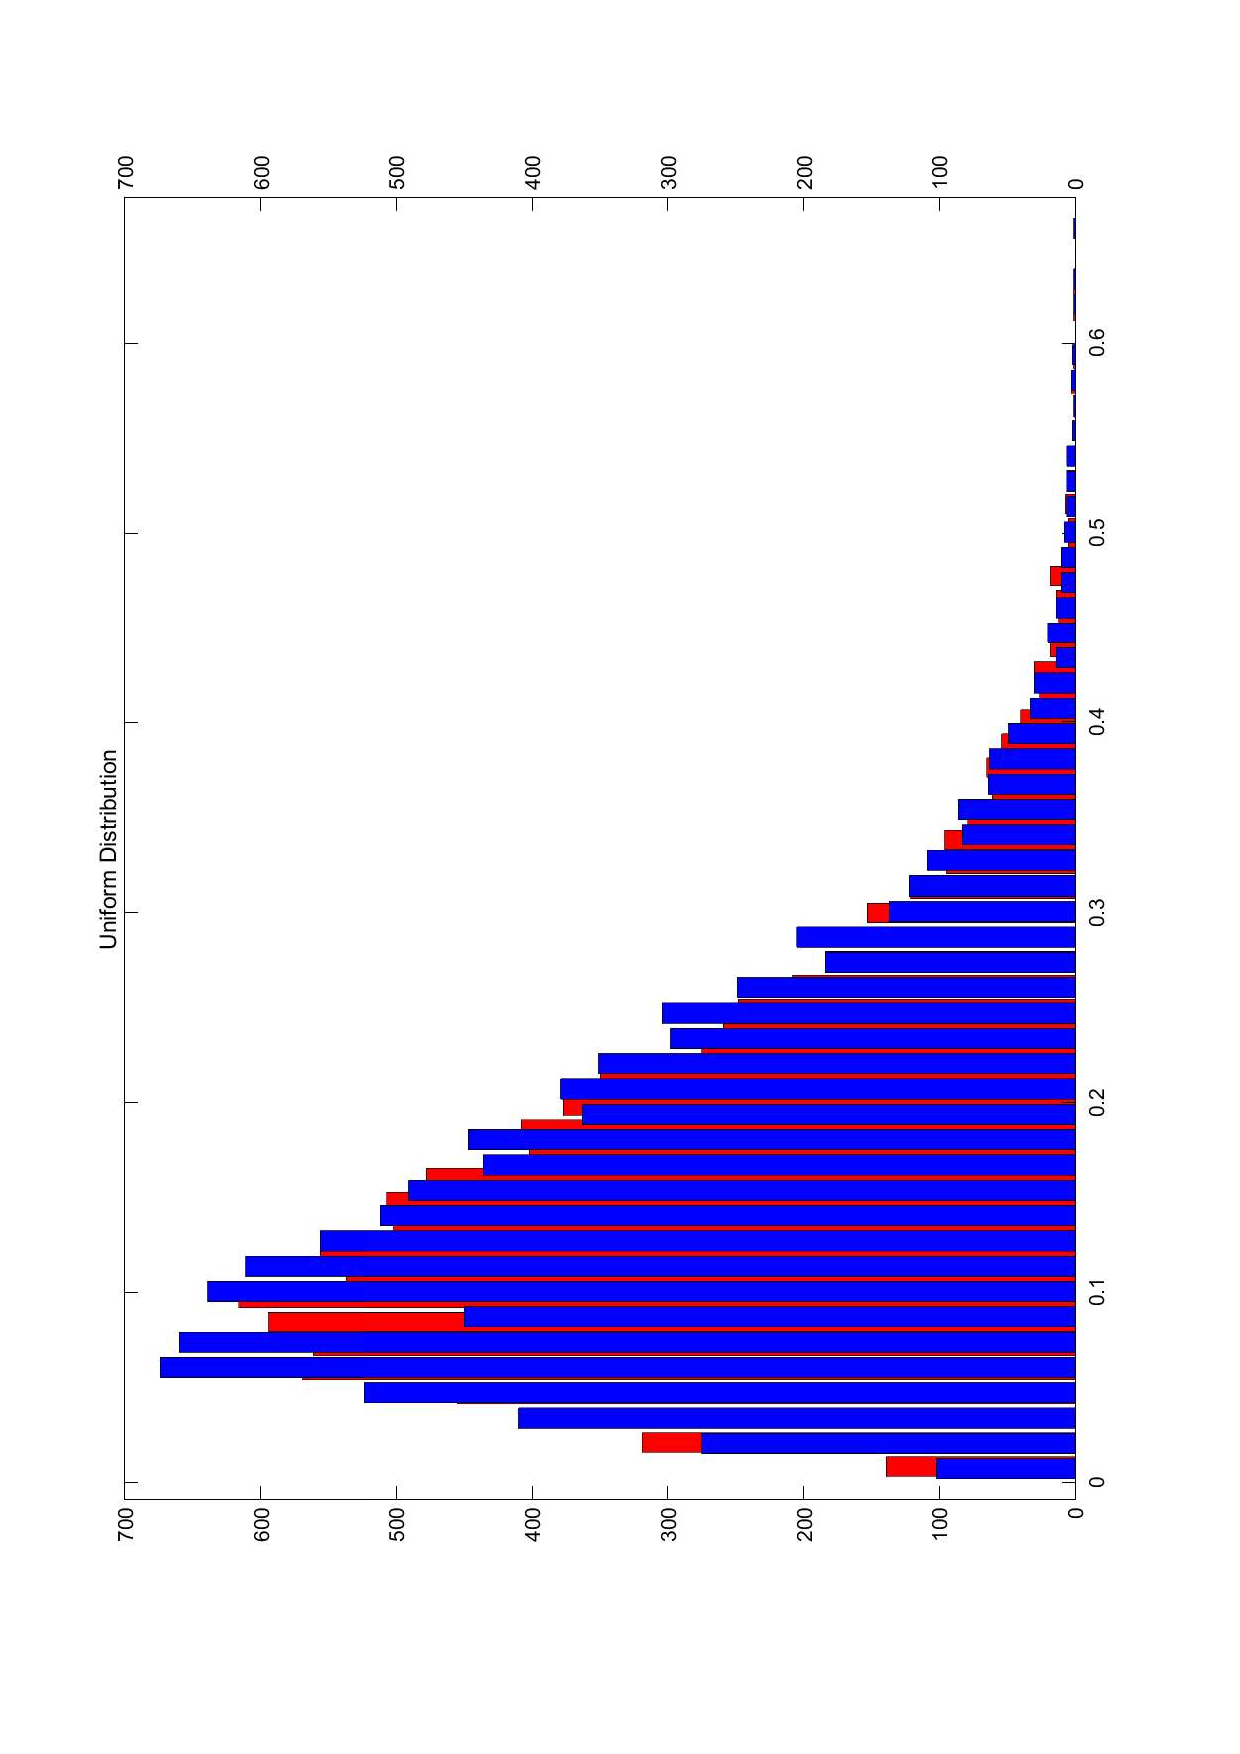
\includegraphics[scale = 0.3, angle=270]{UniformSimulation.pdf}
           \caption{Estimation using Uniform Distribution}
 \end{figure}
\end{frame}

\begin{frame}{Example of Importance Sampling -- Estimate Distribution}
\begin{figure}[ht]
		  \centering
          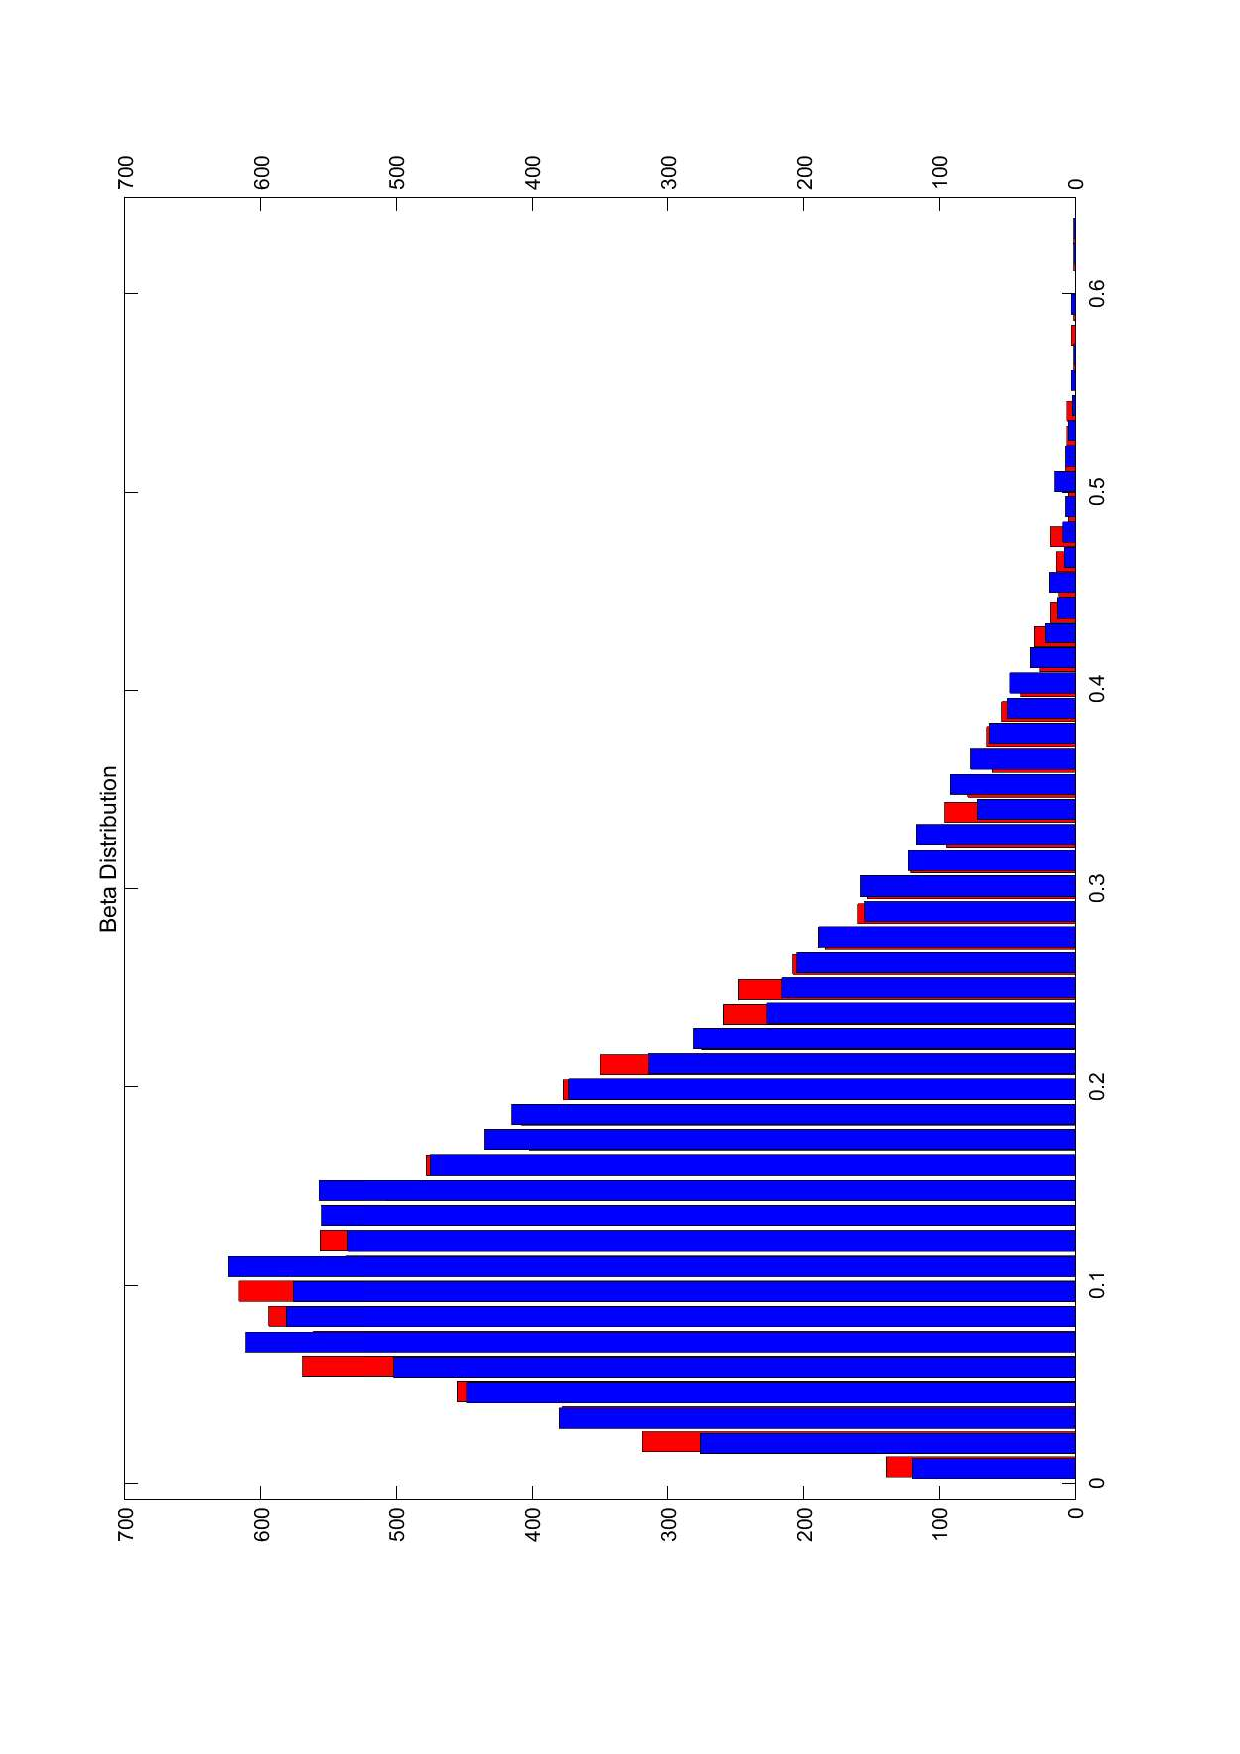
\includegraphics[scale = 0.3, angle=270]{BetaSimulation.pdf}
           \caption{Estimation using Beta Distribution}
 \end{figure}
\end{frame}

\begin{frame}{Example of Importance Sampling -- Calculate Probability}
\begin{example}
Get the expectation value for the function $f(x)$ below, with $x$ value drawn from a standard normal $p(x)=N(0,1)$. \\
\[f(x)=10 e^{-5(x-3)^{4}}\]
\[p(x)=\frac{1}{\sqrt{2 \pi}} e^{-x^{2} / 2}\]First, we calculate the theoretical expectation value using Wolfram Alpha:\\
\[\int_{-\infty}^{\infty} 5 e^{(-3+x)^{4}-\frac{x^{2}}{2}} \sqrt{\frac{2}{\pi}} d x \approx 0.089392379460790\]
\end{example}
\end{frame}

\begin{frame}{Direct Monte Carlo}
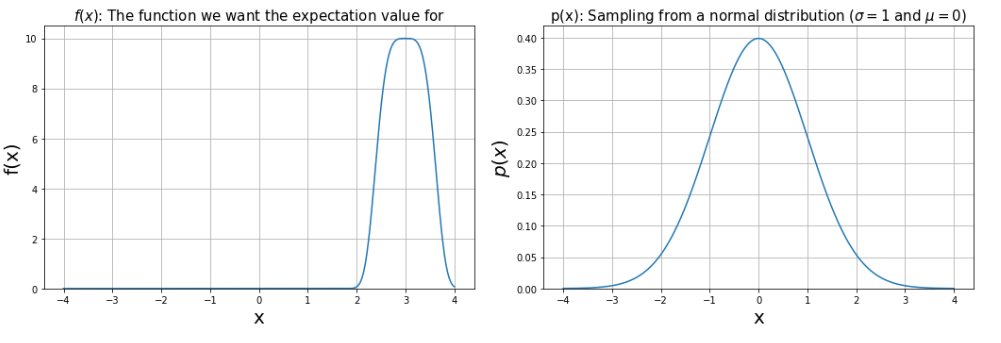
\includegraphics[width=\textwidth*\real{\figfactor}]{ExampleP.png}\\
From the figure above, it's obvious that \textcolor{red}{very few} of the values sampled from $p(x)$ will fall inside the high-value range of the $f(x)$.\\
For $500$ times Monte Carlo simulation:\\
The average expectation value is $0.08920550043488344$.\\
The standard deviation in the average expectation value is $0.024553920882104115$.
\end{frame}

\begin{frame}
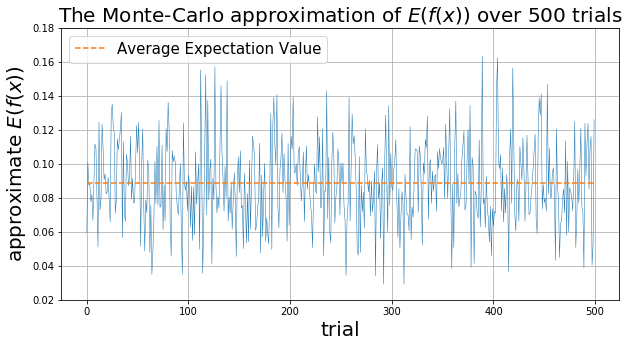
\includegraphics[width=\textwidth*\real{\figfactor}]{DirectMCVariance.png}\\
\end{frame}

\begin{frame}{Importance Sampling}
Now, we choose the second probability density function, $q(x)$, from which sample values are more likely to fall within the high-value range of $f(x)$.\\
For $500$ times Monte Carlo simulation:\\
The average expectation value is $0.0894449539169$.\\
The standard deviation in the average expectation value is $0.00370078677103$.

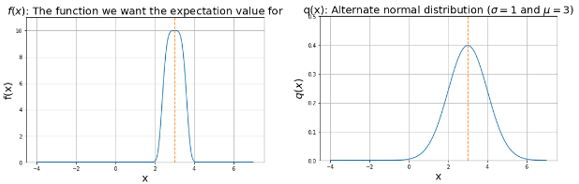
\includegraphics[width=\textwidth*\real{\figfactor}]{q.png}\\
\end{columns}
\end{frame}

\begin{frame}
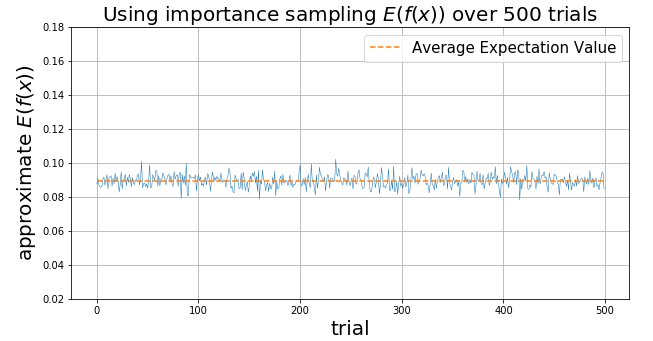
\includegraphics[width=\textwidth*\real{\figfactor}]{ImporSamVariance.png}\\
\end{frame}

\begin{frame}{Pitfall}
\begin{quote}
\textcolor{red}{The tails of the distributions matters!}\\
\end{quote}
While $q(x)$ might be roughly the similar shape as $p(x)$, serious difficulties arise if $q(x)$ gets small much faster than $p(x)$ out in the tail. In such a case, although it is less possible that you will sample a value of $x_{i}$ from the far tails of $q(x)$, your Monte Carlo estimator will take $g\left(x_{i}\right) / h\left(x_{i}\right)$ for such $x_{i}$ may be orders of magnitude larger than the regular values $g\left(x\right) / h\left(x\right)$.
\end{frame}

\begin{frame}{Comparison}
\begin{quote}
\textcolor{red}{Importance Sampling} and \textcolor{red}{Acceptance/Rejection Algorithm} are quite similar ideas. Both of them distort a sample from one distribution in order to sample from another. \\
What is the difference of \textcolor{red}{Importance Sampling} and \textcolor{red}{Acceptance/Rejection Algorithm}?\\
\end{quote}
\end{frame}

\begin{frame}{More Advanced Importance Sampling}
\begin{itemize}
\item Adaptive parametric Importance Sampling.
\item Sequential Importance Sampling.
\item Annealed Importance Sampling
\item SIS with Re-sampling.
\item SIS and Markov Chain Sampling
\end{itemize}
\end{frame}

\begin{frame}{Stratified Sampling    \href{https://en.wikipedia.org/wiki/Stratified_sampling}{[2]}}

 In statistical surveys, when sub-populations within an overall population vary, it could be advantageous to sample each sub-population (stratum) independently. Stratification is the process of dividing members of the population into homogeneous subgroups before sampling. \\
 \textcolor{red}{Mutually Exclusive}: every element in the population must be assigned to only one stratum.\\
 \textcolor{red}{Collectively Exclusive}: no population element can be excluded.
 
\end{frame}

\begin{frame}{Stratified Sampling Procedure}

 1. Divide the population into strata, or groups of individuals that are similar (or homogeneous) in some way that is important to the response.\\
 2. Choose a separate simple random sample (SRS) from each stratum.\\
 3. Combine these SRS's to form a stratified random sample.
 
\end{frame}

\begin{frame}{Stratified Sampling -- Advantages and Disadvantages}

\textcolor{red}{Advantages}:
\begin{itemize}

\item If measurements within strata have lower standard deviation, stratification gives smaller error in estimation.
\item For many applications, measurements become more manageable and/or cheaper when the population is grouped into strata.
\item It is often desirable to have estimates of population parameters for groups within the population
\end{itemize}
\textcolor{red}{Disadvantages}:
Stratified sampling is not useful when the population cannot be exhaustively partitioned into disjoint subgroups.
\end{frame}

\begin{frame}{Stratified Sampling -- Mean and s.d.}

Mean:\\
\[\overline{x}=\frac{1}{N} \sum_{h=1}^{L} N_{h} \overline{x_{h}}\]
Standard error:\\
\[s_{\overline{x}}^{2}=\sum_{h=1}^{L}\left(\frac{N_{h}}{N}\right)^{2}\left(\frac{N_{h}-n_{h}}{N_{h}}\right) \frac{s_{h}^{2}}{n_{h}}\]
Where, $L$ -- Number of strata; $N$ -- the sum of all stratum sizes; $N_{h}$ -- Size of stratum $h$; $\overline{x}_{h}$ -- Sample mean of stratum $h$; $n_{h}$ -- Number of observations in stratum $h$; $s_{h}$ -- Sample standard deviation of stratum $h$.

\end{frame}

\begin{frame}{Stratified Sampling -- Example}

For proportional allocation strategy, the size of the sample in each stratum is taken in proportion to the size of the stratum. Suppose that in a company there are the following staff:
\begin{itemize}

\item male, full-time: $90$
\item male, part-time: $18$
\item female, full-time: $9$
\item female, part-time: $63$
\end{itemize}
Now we want to take sample of 40 staff, stratified according to the above categories.

\end{frame}

\begin{frame}{Stratified Sampling -- Example}
\begin{itemize}

\item male, full-time $=90 \times(40 \div 180)=20$
\item male, part-time $=18 \times(40 \div 180)=4$.
\item female, full-time $=9 \times(40 \div 180)=2$.
\item female, part-time $=63 \times(40 \div 180)=14$.
\end{itemize}

\end{frame}

\begin{frame}{Stratified Sampling -- Example}

\begin{figure}[ht]
		  \centering
          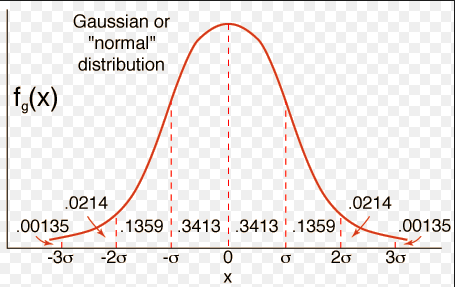
\includegraphics[scale = 0.4]{Normal.png}
           \caption{Gaussian Distribution}
           \href{http://hyperphysics.phy-astr.gsu.edu/hbase/Math/gaufcn.html}{Image Source: Rohlf}
 \end{figure}
 
 If we want to sample $10000$ from the Gaussian distribution above, the sample size in different interval should be:\\
 $[-\infty, -3\sigma]$: $14$; $[-3\sigma, -2\sigma]$: $214$; $[-2\sigma,-\sigma]$: $1359$; $[-\sigma,0]$: $3413$;\\
 $[0,\sigma]$:$3413$; $[\sigma,2\sigma]$:$1359$; $[2\sigma,3\sigma]$: $214$; $[3\sigma, +\infty]$: $14$.
 
 \end{frame}

\begin{frame}{Latin Hypercube Sampling}
Purpose:\\
Recreate the input distribution through less samples.\\
Method:\\
\begin{itemize}
\item The key to this method is \textcolor{red}{stratification} of the input probability distribution.
\item Stratification \textcolor{red}{divides the cumulative curve} into \textcolor{red}{equal} intervals.
\item A sample is then \textcolor{red}{randomly} taken from each interval or "stratification".
\end{itemize}
\end{frame}

\begin{frame}{LHS -- One Dimension}
\begin{figure}[ht]
		  \centering
          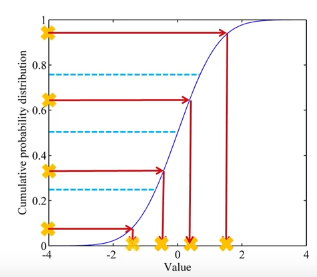
\includegraphics[scale = 0.6]{LHS1D.png}
           \caption{One-dimensional LHS}
           \href{https://www.youtube.com/watch?v=H0RZ1uezuuw}{Image Source: Iman}
 \end{figure}
 Only one sample per stratification.
\end{frame}

\begin{frame}{LHS -- Two Dimension}

 In the context of statistical sampling, a square grid containing sample position is a \textcolor{red}{Latin Square} if and only if there is only \textcolor{red}{one sample} in each row and each column.\\
 A \textcolor{red}{Latin Hypercube} is the generalization of this concept to an arbitrary number of dimensions, whereby each sample is the only one in each axis-aligned heperplane containing it.
 
\end{frame}

\begin{frame}{Comparison}

 \textcolor{red}{Monte Carlo Method -- Memory-less:}\\
 New sample points are generated without taking into account the previously generated sample point. \\
 \textcolor{red}{Latin Hypercube Sampling -- Memory:}\\
 The row and the column the sample point was taken has to be considered to generate the new data points. Spread sample points 'more uniformly' across all the possible values than the basic Monte Carlo methods.
 
\end{frame}

\begin{frame}{LHS -- One Dimension}
\begin{figure}[ht]
		  \centering
          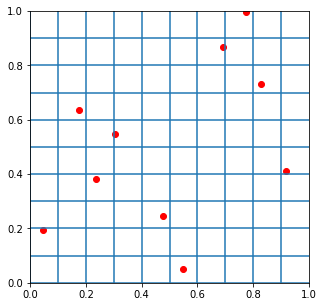
\includegraphics[scale = 0.4]{LHS2D.png}
           \caption{Two-dimensional LHS}
 \end{figure}
 Only one sample in each row and each column.
\end{frame}

\begin{frame}{Reference}
\begin{thebibliography}
\bibitem{[1]} Robert, C., & Casella, G. Monte Carlo statistical methods. Springer Science & Business Media, 2013:  90-91.
\end{thebibiliography}
\end{frame}
%%% Local Variables:
%% y-main"
%%% End:
